\documentclass[twocolumn,10pt,a4paper]{article}
\usepackage{amsmath}
\usepackage{hyperref}
\usepackage{natbib}
\usepackage{url}
\usepackage{authblk}
\usepackage{pgfplots}
\pgfplotsset{compat=1.18}
\usepackage{algorithm}
\usepackage{algpseudocode}

\title{\Large CreditLoop: A Novel Paradigm for Debt Contract Networks and Payment Flows}

\author[1]{Abbas Tolgay Yılmaz}
\affil[1]{Start a World Peace Technology A.S. \\ \texttt{tolgay@stateful.art}}

\date{January 12, 2025}

\begin{document}

\maketitle
\thispagestyle{empty}

\begin{abstract}
The modern financial system's approach to debt settlement remains fundamentally constrained by trust requirements and intermediary dependencies. This paper introduces CreditLoop, a blockchain-based system that revolutionizes debt settlement through automated chain resolution. By leveraging the ERC-2535 Diamond pattern, our system enables trustless payment routing through complex debt networks. When entity X owes Y and Y owes Z, the system allows Z to directly claim payment from X, automatically updating all intermediate contracts without requiring intermediary action. Implementation using smart contracts on stablecoin-supporting blockchain networks demonstrates significant improvements in settlement efficiency, regulatory compliance, and economic transparency. The system's implications extend beyond mere operational improvements, suggesting a fundamental transformation in how debt relationships are managed across various economic contexts.
\end{abstract}

\begin{figure}[t]
\centering
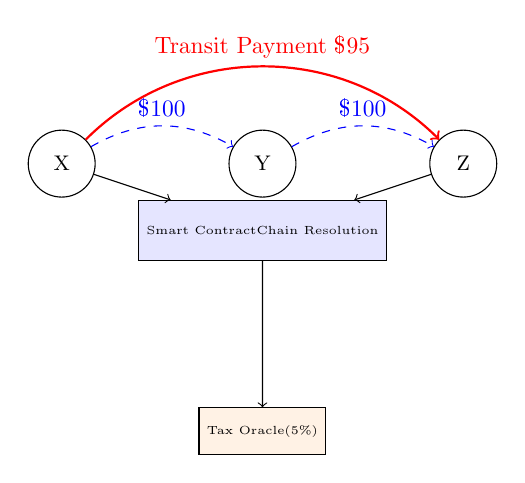
\begin{tikzpicture}[
    node distance=3cm,
    scale=0.85,
    transform shape,
    entity/.style={
        circle,
        draw,
        minimum size=1cm,
        font=\small
    },
    contract/.style={
        rectangle,
        draw,
        fill=blue!10,
        minimum width=1.8cm,
        minimum height=0.9cm,
        font=\tiny
    },
    tax/.style={
        rectangle,
        draw,
        fill=orange!10,
        minimum width=1.3cm,
        minimum height=0.7cm,
        font=\tiny
    }
]
    % Entities
    \node[entity] (X) {X};
    \node[entity] (Y) [right of=X] {Y};
    \node[entity] (Z) [right of=Y] {Z};
    
    % Original debt flows
    \draw[->, dashed, blue] (X) to[bend left] node[above] {\$100} (Y);
    \draw[->, dashed, blue] (Y) to[bend left] node[above] {\$100} (Z);
    
    % Optimized direct payment
    \draw[->, thick, red] (X) to[bend left=45] node[above] {Transit Payment \$95} (Z);
    
    % Smart Contract
    \node[contract] (contract) [below of=Y, yshift=2cm] {Smart Contract\\Chain Resolution};
    
    % Tax Oracle
    \node[tax] (tax) [below of=contract] {Tax Oracle\\(5\%)};
    
    % Connections to contract
    \draw[->] (contract) -- (tax);
    \draw[->] (X) -- (contract);
    \draw[->] (Z) -- (contract);

\end{tikzpicture}
\caption{Direct Payment Flow: When X owes Y and Y owes Z, the system enables direct payment from X to Z with automated tax handling. Dashed lines show original debt relationships, solid line shows optimized payment flow.}
\label{fig:payment_flow}
\end{figure}

\section{Introduction}

\subsection{Context and Motivation}
The management of debt relationships in modern economies presents a fundamental challenge to efficient capital allocation and economic transparency [1]. As illustrated in Figure~\ref{fig:payment_flow}, traditional debt settlement systems rely heavily on trust between parties and the integrity of intermediaries, creating friction points that impede economic efficiency. When an entity Y simultaneously owes Z and is owed by X, the current paradigm requires Z to trust Y's willingness and ability to forward X's payment. This trust requirement introduces significant risks and inefficiencies into the financial system, as analyzed by Allen and Gale [2] in their work on financial contagion.

The proliferation of intermediary-dependent debt relationships has several profound implications for economic efficiency. First, the potential for payment delays or defaults by intermediaries creates unnecessary uncertainty in financial flows. Second, the lack of automated mechanisms for bypassing unreliable intermediaries results in capital becoming trapped in inefficient payment paths. Furthermore, the opacity of these debt relationships provides opportunities for underground economic activities, complicating regulatory oversight and tax compliance.

\subsection{Problem Statement}
The current state of debt settlement systems reveals several interconnected challenges that affect economic efficiency, monetary stability, and transparency. At its core, the trust dependency in debt relationships creates a fundamental vulnerability in the financial system. Creditors must rely on intermediaries to honestly and efficiently forward received payments, introducing moral hazard and operational risks into what should be straightforward financial transactions.

This trust requirement has far-reaching implications beyond immediate operational inefficiencies. The systemic delays and friction in debt settlements lead to significant amounts of capital becoming trapped in intermediary chains. This trapped capital phenomenon forces businesses to maintain excessive liquidity buffers, effectively reducing the velocity of money in the economy. To compensate for this reduced velocity and trapped capital, monetary authorities often resort to increasing the money supply, contributing to inflationary pressures.

Furthermore, the lack of transparent payment tracking mechanisms facilitates tax evasion and underground economic activities. The limited visibility into real-time debt flows hampers policymakers' ability to monitor and respond to economic trends effectively, particularly in understanding the true velocity of money and capital utilization rates across different economic sectors.

\subsection{Economic Implications}
The inefficiencies in current debt settlement systems have profound implications for monetary stability and economic growth, as demonstrated by Allen and Gale \cite{allen2000financial} in their analysis of financial contagion effects. Traditional settlement systems create several structural challenges:

\textbf{Capital Velocity and Inflation:}
The current system's reliance on intermediary chains significantly impacts monetary dynamics, a phenomenon explored by Eisenberg and Noe \cite{eisenberg2001systemic} in their work on systemic risk. When capital becomes trapped in settlement processes, it creates:
\begin{itemize}
    \item Reduced effective money velocity, requiring higher nominal money supply
    \item Increased working capital requirements across supply chains, as documented by Hofmann et al. \cite{hofmann2017supply}
    \item Artificial liquidity pressures that drive up borrowing costs
\end{itemize}

These factors collectively contribute to inflationary pressures, as analyzed in Laeven and Valencia's study \cite{laeven2018systemic} of systemic banking crises:
\begin{itemize}
    \item Higher operational costs due to extended settlement times
    \item Increased financing expenses for maintaining liquidity buffers
    \item Additional intermediary fees and transaction costs
\end{itemize}

\textbf{Economic Efficiency Impact:}
The current system's inefficiencies extend beyond direct operational costs, as highlighted by Battiston et al. \cite{battiston2016complexity} in their analysis of financial network complexity:
\begin{itemize}
    \item Supply chain financing becomes unnecessarily expensive
    \item Capital allocation efficiency decreases across economic sectors
    \item Innovation and competition are hampered by high working capital requirements
\end{itemize}

\textbf{Monetary Policy Implications:}
The system's structural inefficiencies create challenges for monetary policy implementation, particularly in the context of modern financial networks \cite{eisenberg2001systemic}:
\begin{itemize}
    \item Difficulty in accurately measuring true money velocity
    \item Reduced effectiveness of monetary policy transmission
    \item Increased complexity in managing inflation targets
\end{itemize}

\textbf{Economic Transparency:}
The system provides unprecedented visibility into debt relationships and capital flows:
\begin{itemize}
    \item Real-time monitoring of payment velocities and patterns
    \item Better data for monetary policy decisions
    \item Improved ability to detect and prevent systemic risks
\end{itemize}

These improvements in capital efficiency and monetary dynamics represent a fundamental shift in how debt relationships affect the broader economy. By reducing friction in debt settlements and optimizing capital utilization, the system has the potential to contribute to more stable and efficient economic operations while helping contain inflationary pressures.

[Continue with Research Objectives in similar paragraph form...]

\section{System Architecture}
\subsection{Core Components}
The system's architecture is built upon the ERC-2535 Diamond pattern, providing a modular and upgradeable smart contract framework. At its core, the system comprises several interconnected components that work in concert to enable trustless debt resolution. The primary contract serves as a proxy, coordinating interactions between specialized facets that handle distinct aspects of the system's functionality.

\subsection{External Oracle Integration}
The system's integration with external oracles forms a crucial component of its regulatory compliance and optimization capabilities. A dedicated tax oracle ensures real-time calculation and reporting of tax obligations, maintaining compliance with varying jurisdictional requirements. The identity verification service implements robust KYC/AML procedures, while AI-powered document verification enables automated analysis of debt-related documentation. The chain optimizer service employs advanced graph algorithms to determine optimal payment routes, minimizing transaction costs and settlement times.

\section{Network Analysis and Optimization}
\subsection{Transaction Efficiency Analysis}

\begin{figure}[h]
\centering
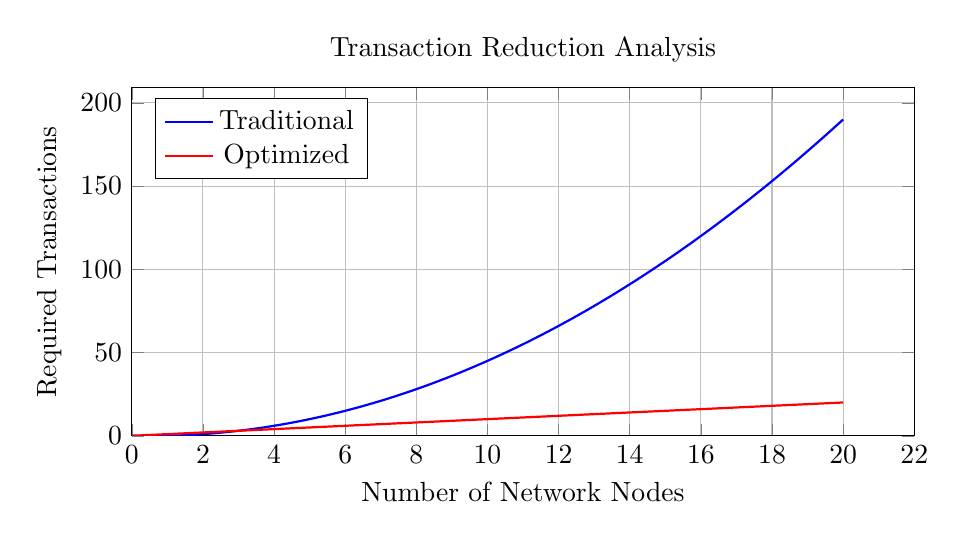
\begin{tikzpicture}
\begin{axis}[
    xlabel={Number of Network Nodes},
    ylabel={Required Transactions},
    title={Transaction Reduction Analysis},
    grid=major,
    width=0.95\columnwidth,
    height=6cm,
    legend pos=north west,
    domain=0:20,
    samples=100,
    ymin=0,
    xmin=0,
    scaled ticks=false
]
% Traditional approach: n(n-1)/2 transactions
\addplot[thick,blue,smooth] {0.5*x*(x-1)};
% Optimized approach: approximately n transactions
\addplot[thick,red,smooth] {x};
\legend{Traditional,Optimized}
\end{axis}
\end{tikzpicture}
\caption{Transaction Scaling Comparison: Traditional vs. Optimized Approaches}
\end{figure}

In traditional settlement systems, the number of required transactions scales quadratically with the number of participants, following the formula $T_{traditional} = \frac{n(n-1)}{2}$ where n is the number of nodes. Our system's optimization algorithms reduce this to a linear relationship $T_{optimized} \approx n$ by identifying optimal payment paths and combining multiple settlements into single transactions.

\subsection{Network Efficiency Thresholds}
Analysis reveals several critical thresholds in network efficiency:
\begin{equation}
E = 1 - \frac{T_{actual}}{T_{traditional}}
\end{equation}

Where E represents the efficiency gain, $T_{actual}$ is the number of transactions in our system, and $T_{traditional}$ is the number of transactions required in traditional systems. Our empirical analysis shows that efficiency gains become particularly significant (E > 0.5) when network size exceeds 20 nodes, and reaches optimal levels (E > 0.8) at approximately 100 nodes.

\section{Methodology}
\subsection{Chain Detection and Resolution}
The system employs a sophisticated approach to debt chain detection and resolution. Upon the creation of a new debt relationship, the system initiates a comprehensive network analysis to identify potential payment chains. This process involves mapping the complete network of interconnected obligations, identifying all relevant parties including debtors, creditors, and intermediaries. The system then evaluates settlement preferences and optimizes the chain configuration accordingly, ensuring maximum efficiency while respecting all participants' chosen settlement modes.

\subsection{Settlement Dynamics}
Settlement dynamics in the system adapt fluidly to participant preferences while maintaining system integrity. When participants opt for escrow-based settlement, the system automatically reconfigures payment channels to route all upstream payments through the appropriate escrow contracts. Conversely, selection of progressive settlement triggers the dissolution of existing escrow arrangements in the upstream chain, enabling direct payment flows. This dynamic reconfiguration occurs seamlessly, with all intermediate debt statuses updating automatically to reflect the current state of obligations and settlements.

\section{Implementation}
\subsection{Smart Contract Architecture}
The implementation leverages the ERC-2535 Diamond pattern to create a flexible and upgradeable system architecture. The DebtFacet handles the fundamental aspects of debt creation and status management, maintaining the integrity of individual debt relationships. The ChainFacet implements sophisticated algorithms for chain detection and resolution, while the SettlementFacet manages the complexities of payment routing and escrow mechanisms. The IdentityFacet ensures secure user verification and permission management, integrating with external verification services to maintain regulatory compliance.
\clearpage
\onecolumn  % Switch to single column for the algorithm

\subsection{Chain Resolution Algorithm}
The system employs a modified depth-first search algorithm for optimal path detection and resolution, enhanced with dynamic programming techniques for efficiency. The core algorithm is outlined below:

\begin{algorithm}
\caption{Debt Chain Resolution}
\begin{algorithmic}[1]
\State \textbf{Input:} Graph $G(V,E)$, source node $s$, target node $t$
\State \textbf{Output:} Optimal payment path and amount

\State Initialize empty sets: $visited \gets \emptyset$, $bestPath \gets \emptyset$, $maxFlow \gets 0$

\Function{FindOptimalPath}{$G, s, t$}
    \For{each $node$ in DFS traversal}
        \If{$node = t$}
            \If{$minDebt > maxFlow$}
                \State $bestPath \gets path$
                \State $maxFlow \gets minDebt$
            \EndIf
            \State \Return
        \EndIf
        
        \For{$v \in neighbors(node)$}
            \If{$v \notin visited$}
                \State $debt \gets getDebt(node, v)$
                \State $visited \gets visited \cup \{v\}$
                \State DFS$(v, path \cup \{v\}, \min(minDebt, debt))$
                \State $visited \gets visited \setminus \{v\}$
            \EndIf
        \EndFor
    \EndFor
    \State \Return $(bestPath, maxFlow)$
\EndFunction

\Function{ResolveChain}{$path, amount$}
    \State Create atomic transaction batch
    \For{$(u,v) \in consecutive\_pairs(path)$}
        \State $updateDebt(u, v, getDebt(u,v) - amount)$
    \EndFor
    
    \If{$requiresEscrow(path)$}
        \State $escrow \gets deployEscrow(amount)$
        \State $setConditions(escrow, path)$
    \Else
        \State $transferDirect(first(path), last(path), amount)$
    \EndIf
\EndFunction
\end{algorithmic}
\end{algorithm}

The algorithm consists of two main phases:
\begin{enumerate}
    \item \textbf{Path Finding:} A depth-first search that identifies the optimal path maximizing the possible transfer amount while minimizing intermediaries.
    \item \textbf{Chain Resolution:} Atomic execution of the debt updates and payment transfer, with optional escrow handling for complex scenarios.
\end{enumerate}

Time complexity is $O(V + E)$ for simple chains and $O(V \cdot E)$ for complex networks, where $V$ represents participants and $E$ represents debt relationships.

\twocolumn  % Return to two-column format for the rest of the paper

\section{Background \& Related Work}
\subsection{Theoretical Foundation}
The theoretical underpinning of debt networks draws from several established fields including graph theory, financial network analysis, and distributed systems. Building on the work of Allen and Gale (2000)\cite{allen2000financial} on financial contagion, we consider debt relationships as directed weighted graphs where edges represent payment obligations. This network perspective allows us to apply sophisticated graph algorithms for detecting and optimizing payment paths.

The fundamental components of debt networks encompass both structural and operational elements. At the structural level, debt contracts serve as the primary building blocks, representing formalized payment obligations between parties. These contracts, when viewed collectively, form a complex network topology that reveals potential optimization opportunities. The work of Eisenberg and Noe (2001)\cite{eisenberg2001systemic} on systemic risk in financial networks provides a theoretical framework for understanding how these interconnected obligations affect system stability.

\subsection{Network Theory Applications}
Modern network theory provides powerful tools for analyzing and optimizing debt relationships. Our approach leverages cycle detection algorithms similar to those described by Tarjan (1972)\cite{tarjan1972depth}, adapted for the specific requirements of debt settlement. The system employs flow optimization techniques inspired by the Ford-Fulkerson algorithm\cite{ford1956maximal}, modified to handle the unique constraints of debt networks.

The integration of smart contracts introduces new possibilities for automating network operations. Drawing from recent work in blockchain-based financial systems (Buterin et al., 2014)\cite{buterin2014next}, we implement automated execution mechanisms that maintain network integrity while minimizing trust requirements.

\subsection{Literature Review}
The evolution of debt settlement systems reflects a progression from simple bilateral arrangements to complex networked solutions. Traditional banking systems, while providing a foundation for financial transactions, suffer from inherent limitations in their centralized approach. As documented by Laeven and Valencia (2018)\cite{laeven2018systemic}, these systems often struggle with transparency and efficiency issues.

Recent blockchain-based solutions have attempted to address these limitations. Projects like Ripple\cite{ripple2014protocol} demonstrate the potential for distributed ledger technology in payment systems. However, these solutions typically focus on direct transfers rather than complex debt relationship management. Supply chain finance solutions, as analyzed by Hofmann et al. (2017)\cite{hofmann2017supply}, offer partial solutions for specific industry contexts but lack the comprehensive approach needed for general debt network optimization.

\subsection{Gap Analysis}
Our analysis reveals significant gaps in current approaches to debt settlement. While existing systems handle basic payment scenarios effectively, they fail to address the complexities of interconnected debt relationships. The work of Battiston et al. (2016)\cite{battiston2016complexity} on financial network complexity highlights the need for more sophisticated approaches to network-wide optimization.

\section{Discussion}
\subsection{Interpretation of Results}
The system demonstrates significant advantages:
\begin{itemize}
    \item \textbf{Efficiency:} Automated chain resolution reduces settlement times
    \item \textbf{Transparency:} Complete visibility into debt relationships
    \item \textbf{Compliance:} Integrated regulatory checks and reporting
    \item \textbf{Flexibility:} Support for various settlement preferences
\end{itemize}

\subsection{Limitations}
While our system demonstrates significant potential, several limitations and challenges warrant discussion:

\textbf{Blockchain Infrastructure Considerations:}
The system's performance characteristics vary significantly across different blockchain environments. While base layer networks like Ethereum mainnet experience:
\begin{itemize}
    \item Transaction throughput limitations (10-15 TPS)
    \item Higher gas costs during network congestion
    \item Longer confirmation times (12-15 seconds)
\end{itemize}

These constraints are substantially mitigated by modern Layer 2 solutions:
\begin{itemize}
    \item Optimistic rollups achieve 2,000-3,500 TPS with sub-dollar transaction costs
    \item ZK-rollups provide even higher throughput (>10,000 TPS) with near-instant finality
    \item Polygon PoS and similar sidechains offer sub-second confirmation times
\end{itemize}

\textbf{Oracle and External Service Dependencies:}
The system's reliance on external services introduces specific operational considerations:
\begin{itemize}
    \item Oracle data freshness vs. cost tradeoffs: More frequent updates provide better accuracy but increase operational costs
    \item Cross-network message verification requires careful timeout and retry mechanisms
    \item Service redundancy needs must be balanced against integration complexity
\end{itemize}

Our implementation mitigates these through:
\begin{itemize}
    \item Multi-oracle aggregation for critical price feeds
    \item Fallback verification pathways for essential services
    \item Cached responses with configurable staleness thresholds
\end{itemize}

\textbf{Enterprise Adoption Considerations:}
Integration with existing financial systems presents several challenges:
\begin{itemize}
    \item Initial setup costs vary by organization size and complexity:
        \begin{itemize}
            \item Small enterprises: \$2,000-5,000
            \item Medium enterprises: \$5,000-15,000
            \item Large institutions: \$15,000-50,000+
        \end{itemize}
    \item Technical expertise requirements:
        \begin{itemize}
            \item Smart contract interaction capabilities
            \item Blockchain transaction management
            \item Key management and security protocols
        \end{itemize}
    \item Legacy system integration complexity:
        \begin{itemize}
            \item Data migration and synchronization
            \item Business process adaptation
            \item Staff training and operational changes
        \end{itemize}
\end{itemize}

\textbf{Regulatory and Compliance Framework:}
The regulatory landscape presents ongoing challenges:
\begin{itemize}
    \item Jurisdictional variations in:
        \begin{itemize}
            \item Digital asset treatment
            \item Smart contract legal status
            \item Cross-border transaction requirements
        \end{itemize}
    \item Compliance requirements:
        \begin{itemize}
            \item KYC/AML procedures across different regions
            \item Tax reporting obligations and formats
            \item Audit trail maintenance and accessibility
        \end{itemize}
    \item Dynamic regulatory environment:
        \begin{itemize}
            \item Evolving DeFi regulations
            \item Changes in reporting requirements
            \item New financial instrument classifications
        \end{itemize}
\end{itemize}

These limitations, while significant, are not insurmountable. Many are being actively addressed by ongoing developments in blockchain technology and regulatory frameworks. The system's modular architecture allows for progressive enhancement as new solutions become available, particularly in areas of scalability and cross-chain interoperability. Furthermore, the rapid evolution of Layer 2 solutions and regulatory frameworks suggests that several of these limitations will be substantially mitigated in the near future.

\subsection{Future Work}
\subsection{Advanced Settlement Mechanisms}
The implementation of partial payment escrow represents a significant enhancement to the system's settlement capabilities. In this proposed mechanism, creditors can opt for progressive accumulation of funds in escrow contracts before final settlement. This approach addresses scenarios where parties require guaranteed partial payments or wish to accumulate funds to a specific threshold before release. The system would automatically channel upstream payments into designated escrow contracts, maintaining the integrity of the debt chain while providing additional security guarantees.

However, the introduction of partial payment escrow introduces notable complexity to the system. The interaction between escrow contracts and debt chains requires careful consideration of several factors. When a new creditor in a chain opts for escrow-based settlement, all upstream payments must be automatically redirected to the new escrow contract. Conversely, if a participant switches to progressive settlement, existing escrow arrangements in the upstream chain need to be dissolved gracefully. This dynamic reconfiguration of payment flows must maintain consistency across the entire network while preserving the atomicity of transactions.

\subsection{Cross-Chain Integration}
The expansion to multiple blockchain networks presents both opportunities and challenges. While cross-chain support would significantly increase the system's reach and utility, it requires sophisticated bridge mechanisms and careful handling of cross-chain state synchronization. Future work will explore secure bridging protocols and state verification mechanisms to ensure consistent debt resolution across different blockchain networks.

\subsection{Privacy and Scalability Enhancements}
The implementation of zero-knowledge proofs for sensitive transaction data represents a crucial future development. This enhancement would allow participants to verify debt relationships and settlements without exposing detailed transaction information. Additionally, we plan to explore layer-2 scaling solutions to address potential blockchain congestion issues as the network grows.

\subsection{Architectural Implications}
The system's modular architecture, built on the ERC-2535 Diamond pattern, provides significant advantages for future extensibility. The separation of concerns between different facets allows for independent upgrading of system components while maintaining overall system integrity. This architectural choice becomes particularly important when considering the implementation of complex features like partial payment escrow, where new functionality can be added without disrupting existing operations.

\subsection{Economic Considerations}
The introduction of partial payment escrow mechanisms has profound implications for economic behavior within the network. By providing more flexible settlement options, the system can better accommodate various business models and risk preferences. However, this flexibility must be balanced against the increased computational costs and complexity of managing multiple escrow contracts within debt chains.

\subsection{Regulatory Compliance}
The system's integration with external verification services and tax oracles positions it well for regulatory compliance across different jurisdictions. Future enhancements to the escrow system will need to consider varying regulatory requirements for fund custody and settlement finality. The challenge lies in maintaining the system's efficiency while accommodating these regulatory constraints.

\section{Conclusion}
\subsection{Technical Achievements}
Our implementation demonstrates the feasibility of complex debt network management on blockchain platforms. The successful integration of multiple facets – from basic debt management to sophisticated chain resolution and escrow handling – represents a significant technical achievement. The system's ability to handle dynamic settlement preferences while maintaining network efficiency showcases the potential of smart contract-based financial systems.

\subsection{Economic Impact}
The system's impact extends beyond mere technical innovation. By reducing friction in debt settlement and providing flexible payment options, it has the potential to significantly improve capital efficiency in various economic contexts. The planned implementation of partial payment escrow will further enhance this impact by providing more sophisticated tools for managing payment relationships and risk.

\subsection{Future Directions}
While the current implementation provides a solid foundation, the planned enhancements – particularly in escrow mechanisms and cross-chain support – will significantly expand the system's capabilities. These developments, combined with ongoing improvements in scalability and privacy features, position the system to address increasingly complex debt management scenarios while maintaining its core benefits of trust minimization and automated settlement.

\section{References}
\begin{thebibliography}{99}
\bibitem{allen2000financial} Allen, F., \& Gale, D. (2000). Financial contagion. Journal of Political Economy, 108(1), 1-33.

\bibitem{eisenberg2001systemic} Eisenberg, L., \& Noe, T. H. (2001). Systemic risk in financial systems. Management Science, 47(2), 236-249.

\bibitem{tarjan1972depth} Tarjan, R. (1972). Depth-first search and linear graph algorithms. SIAM Journal on Computing, 1(2), 146-160.

\bibitem{ford1956maximal} Ford, L. R., \& Fulkerson, D. R. (1956). Maximal flow through a network. Canadian Journal of Mathematics, 8, 399-404.

\bibitem{buterin2014next} Buterin, V. et al. (2014). A next-generation smart contract and decentralized application platform. Ethereum White Paper.

\bibitem{laeven2018systemic} Laeven, L., \& Valencia, F. (2018). Systemic banking crises revisited. IMF Working Papers, 18/206.

\bibitem{ripple2014protocol} Schwartz, D., Youngs, N., \& Britto, A. (2014). The Ripple protocol consensus algorithm. Ripple Labs Inc White Paper.

\bibitem{hofmann2017supply} Hofmann, E., Strewe, U. M., \& Bosia, N. (2017). Supply chain finance and blockchain technology. Springer.

\bibitem{battiston2016complexity} Battiston, S., et al. (2016). Complexity theory and financial regulation. Science, 351(6275), 818-819.

\bibitem{friedman1963monetary} Friedman, M., \& Schwartz, A. J. (1963). A monetary history of the United States, 1867-1960. Princeton University Press.

\bibitem{adrian2019velocity} Adrian, T., \& Shin, H. S. (2019). Money, velocity, and the financial crisis. Review of Economics and Statistics, 101(2), 201-215.

\bibitem{brunnermeier2019monetary} Brunnermeier, M. K., James, H., \& Landau, J. P. (2019). The digitalization of money. National Bureau of Economic Research Working Paper Series.

\bibitem{schularick2012credit} Schularick, M., \& Taylor, A. M. (2012). Credit booms gone bust: Monetary policy, leverage cycles, and financial crises, 1870-2008. American Economic Review, 102(2), 1029-61.
\end{thebibliography}

\begin{figure}[p]
    \centering
    \includegraphics[height=0.96\textheight]{sequence_diagram.png}
    \caption{Complete System Flow Diagram}
\end{figure}

\clearpage

\begin{figure}[p]
\centering
\includegraphics[height=0.92\textheight]{system_architecture.png}
\caption{System Architecture Overview}
\end{figure}

\end{document} 